%\documentclass[11pt, onecolumn, conference]{IEEEtran}
\documentclass[12pt, conference]{IEEEtran}
\IEEEoverridecommandlockouts
% The preceding line is only needed to identify funding in the first footnote. If that is unneeded, please comment it out.
\usepackage{cite}
\usepackage{amsmath,amssymb,amsfonts}
\usepackage{algorithmic}
\usepackage{graphicx}
\usepackage{textcomp}
\usepackage{xcolor}
\usepackage{array}
\usepackage[font=large,labelfont=bf]{caption}
\def\BibTeX{{\rm B\kern-.05em{\sc i\kern-.025em b}\kern-.08em
    T\kern-.1667em\lower.7ex\hbox{E}\kern-.125emX}}
\begin{document}

\title{Distributed Mutual Exlcusion Algorithms: Implementation of Multicast in
the IEC61499 standard\\
{\footnotesize COMPSYS 725: Distributed Cyber-Physical Systems}
}

\author{\IEEEauthorblockN{Matt Eden}
\IEEEauthorblockA{\textit{Department of Electrical, Computer and Software
Engineering} \\
\textit{University of Auckland}\\
Auckland, New Zealand \\
mede607@aucklanduni.ac.nz}
}

\maketitle

%\begin{abstract}
%\end{abstract}

%\begin{IEEEkeywords}
%central server, ring token, multicast, mutual exclusion, distributed systems
%\end{IEEEkeywords}

\section{Overview}
Alongside other mutual exclusion algorithms for
a baggage handling system, the \textit{Multicast} algorithm was implemented to control
access to one of three critical sections (CS). The CS in question is
pictured in Figure~\ref{fig:baggage-system} as `Critical Section 3'. As can be
seen, the bags from conveyors 8 and 11 feed into conveyor 9, so the purpose of
the algorithm is to control which of those two conveyors is allowed to send
a bag onto conveyor 9. 
\section{Implementation}
A general overview of the \textit{Multicast} algorithm can be seen in
Figure~\ref{fig:multicast}. A short summary would be that a process wishing to
enter the CS must seek approval from all other processes in the
system. In the case of this system, there are only two processes which makes
the implementation quite simple and to some extent overengineered.

The request for a process to enter the CS is triggered by `photo
eyes' (PEs); essentially sensors which detect when a bag has crossed a certain point.
These are active low, so when the signal stops being high that indicates a bag
has crossed the sensor. The PEs of interest for the CS I'm
concerned with are PE8, PE11 and PE14. Each of the two `input' conveyors
are concerned with two photo eyes; their own and PE14, which represents the
CS.

Before diving into the ECC, it may be helpful to consider the function block shown in
Figure~\ref{fig:function-block}. Several of the inputs and outputs are not unique to the
implementation of the \textit{Multicast} algorithm, but those that are of
importance are described in Table~\ref{tab:multicast-io}. In addition to
those, there are a couple of internal variables used; namely \texttt{HAS\_TOKEN}
and \texttt{LAM\_CLOCK}. The former is simply a flag to indicate whether
a conveyor has been given access to the CS, and the latter is the
Lamport clock (LC) that is used for the \textit{Multicast} algorithm. 

The ECC for the function block is
given in Figure~\ref{fig:multicast-ecc}. In it, \texttt{PECS} stands for `Photo Eye CS' and refers to PE14, with
\texttt{PE} referring to either PE8 or PE11 depending on the conveyor. 
In the ECC, there are two `paths' that represent the implementation of the \textit{Multicast} algorithm. One path is concerned with
replying to requests, and another is concerned with making those requests.
Firstly, consider the \texttt{REC\_REQ\&!HAS\_TOKEN} guard condition in the top
right of the ECC. This represents when the conveyor is receiving a request from
another conveyor, or in more literal terms it has received a request and is not
in the CS. Note that we are not concerned with what happens when
the conveyor has made a request and then received a request, as that is handled
elsewhere in the ECC. Upon receiving this request, there is then a check
performed of the LC (i.e. \texttt{LC\_CHECK}) which updates the
LC of the conveyor that received the request with the LC
of the conveyor that sent the request. This implementation is only concerned
with two conveyors, so this check is a very straightforward process. However,
to generalise this to \textit{N} conveyors may be difficult as each conveyor
would need to know the LC of every other conveyor.

Moving on now to how requests are handled with the left-most path in the
ECC, see that the initial guard condition is given as \texttt{REQ\&!PE};
simply watching for the triggering of the PE by a bag. This then leads
to a state called \textit{MULTICAST}, which causes the action
\texttt{MAKE\_REQUEST} and the event \texttt{MULTICAST} to trigger. The latter
of which simply feeds into an input in the other conveyor, at which point it
moves through the aforementioned process about receiving a request. The action
\texttt{MAKE\_REQUEST} has a few responsibilities. The first of which being to
stop the motor, so that the bag stops moving on the conveyor while it waits to
be let in to the CS. The second of which is to update the LC; 
both internally and in terms of the output. At this point, there are two
possibilities. Either (a) a reply is received from the other conveyor or (b)
a request is received from the other conveyor. For the case of (a) it will move
to the next state, but in the case of (b) there needs to be a check for the
\texttt{TRUMP} variable. The approach by the \textit{Multicast} algorithm for
situations where two requests are sent around the same time is to pick
a process and give priority; that is to say one process `trumps' over the
other. This is reflected by the \texttt{TRUMP} variable, with the conveyor that
has been labelled as the `trump' able to progress to the next state, while the
other conveyor must wait for a reply. Note that this also avoids a deadlock
state where both conveyors wait for a reply from the other by allowing one to
move ahead without a reply.

Having received a reply, the conveyor moves onto a \textit{TEMP} state which
serves to trigger the \texttt{ENTER\_CS} action that turns the motor back on
and sets the internal flag variable \texttt{HAS\_TOKEN} to true. The guard
condition of \texttt{REQ\&PE} which prevents moving to the next state is in
place to account for cases where two bags are quite close together on the
conveyor; this approach means the bag needs to leave the first PE before
it can then trigger the PE for the CS and be released. At
this point in the ECC, there is a bag in the CS; it has achieved
\textit{ACCESS}. As just mentioned the bag exits the CS, or is
\textit{RELEASED}, when it triggers the PE represented by \texttt{PECS}.
At which point the action \texttt{EXIT\_CS} is triggered, the flag variable
\texttt{HAS\_TOKEN} is set to false and the event \texttt{ACK} is triggered as
a reply to the other conveyor to satisfy any requests made.

The final element of this ECC to consider is the \textit{WAIT} state. This
handles situations for a bag on the same conveyor wanting to enter the critical
section when there is already a bag in the CS; evidenced by the
guard condition \texttt{REQ\&HAS\_TOKEN\&!PE}. For this situation, we want to
stop the motor, wait until the CS is available and then move back
to the \textit{ACCESS} state. This allows the waiting bag (from the same
conveyor) to move on to the CS once the previous bag has left.

\section{Conclusion}
Overall, this implementation of the \textit{Multicast} algorithm ensures that all three requirements of mutual
exclusion are satisfied: safety, liveness and fairness. 

\begin{table*}[t]
\caption{Overview of relevant inputs and outputs to multicast function block}
\begin{center}
  \begin{tabular}{|l|l|}
\hline
    Input/Output & Description \\
\hline
    REC\_REQ & Receives a request from another process wishing to enter the
    CS\\
\hline
    REPLY & Receives a reply from a process, acknowledging a request \\
\hline
    PE & Represents the photo eye for that conveyor \\
\hline
    PECS & Represents the photo eye for the CS\\
\hline
    LC & Takes in the lamport clock of the other conveyor \\
\hline
    TRUMP & Indicates whether this conveyor will `trump' over another in times
    of conflict\\
\hline
    ACK & Sends out an acknowledgement upon receiving a request from another
    process \\
\hline
    MULTICAST & Sends out a request to indicate desire to enter critical
    section \\
\hline
    LC\_OUT & Outputs the lamport clock of this conveyor \\
\hline
\end{tabular}
\label{tab:multicast-io}
\end{center}
\end{table*}

\begin{figure}[htbp]
  \centerline{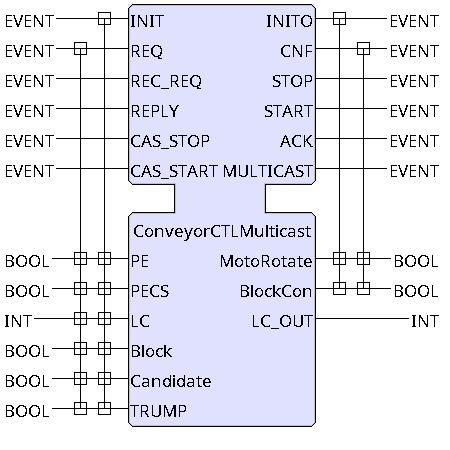
\includegraphics[width=0.5\textwidth]{function-block.png}}
  \caption{The function block for a conveyor using multicast}
\label{fig:function-block}
\end{figure}

\begin{figure*}[htbp]
  \centerline{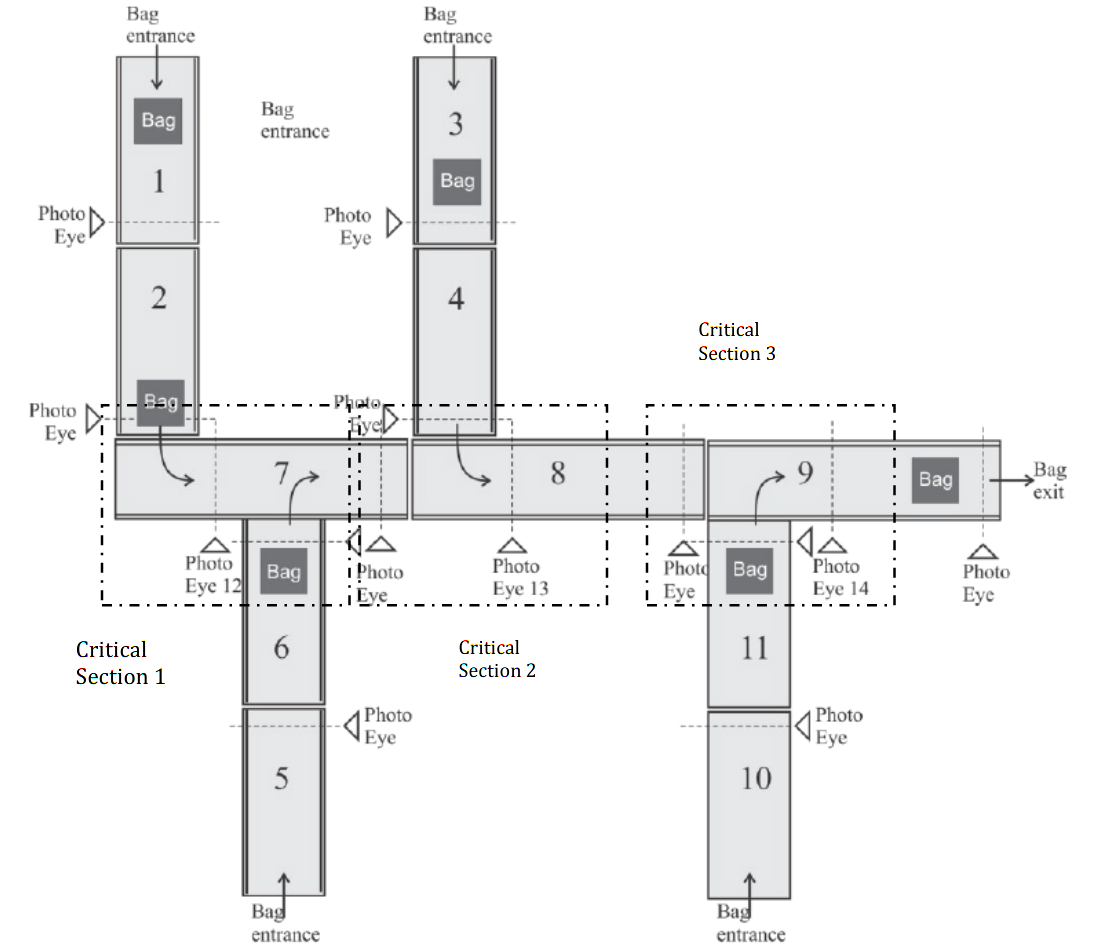
\includegraphics[width=1.0\textwidth]{baggage-handling-system.png}}
  \caption{The baggage handling system}
\label{fig:baggage-system}
\end{figure*}

\begin{figure*}[htbp]
  \centerline{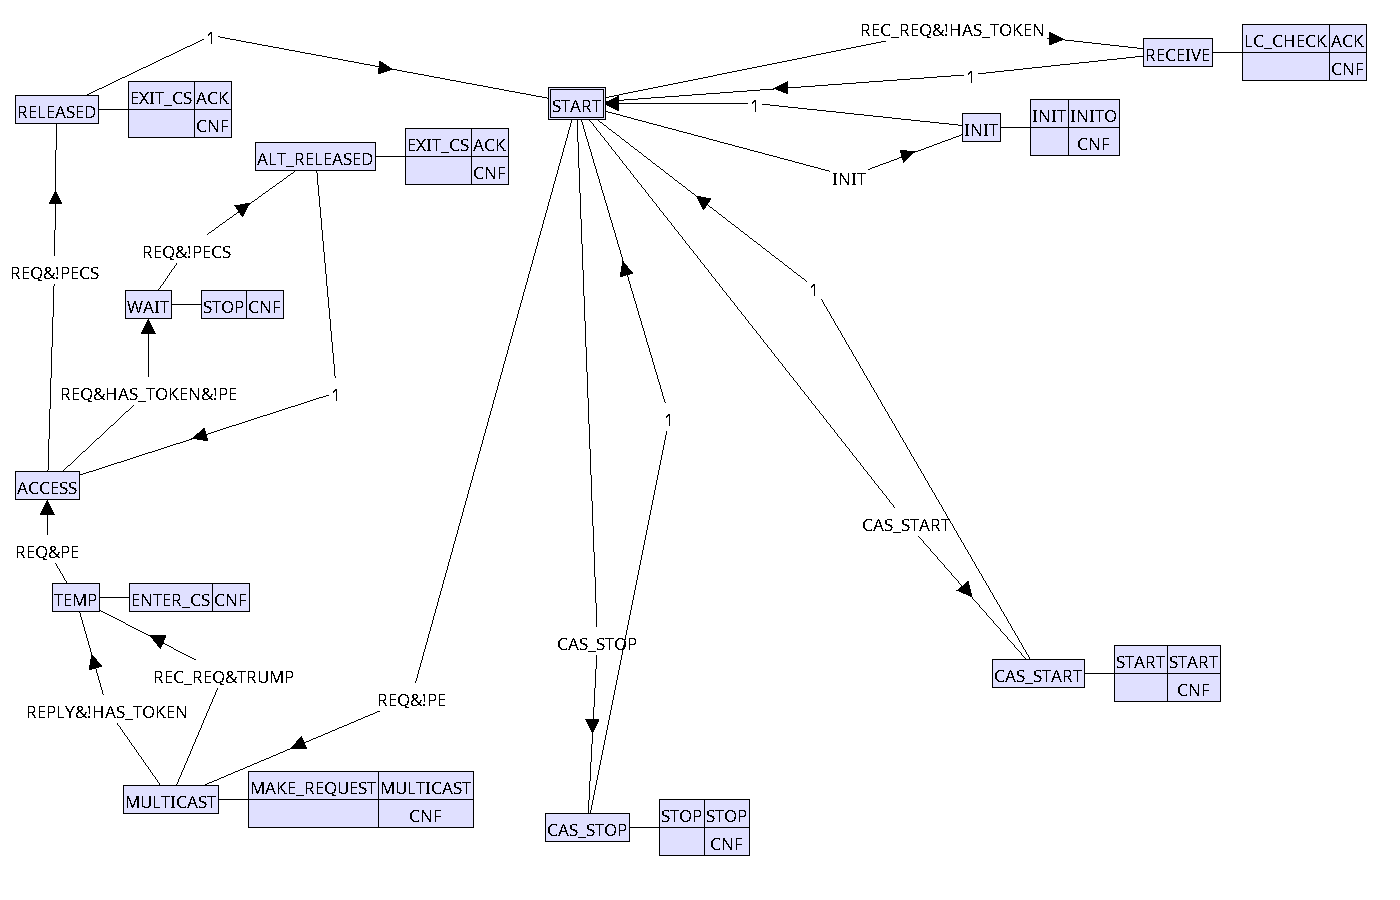
\includegraphics[width=1.0\textwidth]{multicast-ecc.png}}
  \caption{The ECC of the multicast implementation}
\label{fig:multicast-ecc}
\end{figure*}

\begin{figure*}[htbp]
  \centerline{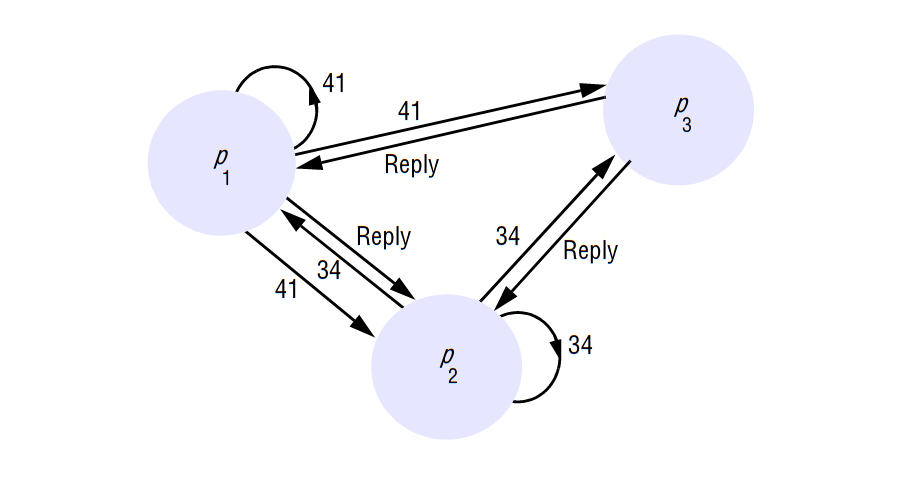
\includegraphics[width=0.75\textwidth]{multicast.png}}
  \caption{\large An example of the \textit{Multicast} algorithm}
\label{fig:multicast}
\end{figure*}

\begin{figure*}[htbp]
  \centerline{\includegraphics[width=1.0\textwidth]{725-meme.png}}
  \caption{A Marie Kondo themed variant of the infamous Drake Hotline Bling
  meme}
\label{fig:meme}
\end{figure*}

\section*{Acknowledgement}
This report acknowledges the teachings of Dr. Avinash Malik and Ms. Jesin James
in the course COMPSYS 725: Distributed Cyber-Physical Systems taught at the
University of Auckland in Semester Two of the year 2020.

\end{document}
